As outlined in Sections~\ref{sec:esteig} and~\ref{sec:opteig}, the main technical barriers to OED using EIG maximisation are the estimation and optimisation of EIG. Here we address methods for estimation.

\section{Variational optimal experiment design}
\label{sec:voed}
\textbf{Note}: This section is broadly based on a paper recently submitted to the NIPS BDL workshop; we intend to submit a longer version to ICML 2019.
\bigskip

The core contribution of this section is to introduce efficient variational methods for EIG estimation that are applicable to a wide variety of models.
The first method, which is related to amortised variational inference \cite{dayan1995helmholtz,kingma2014auto,paige2016inference,rezende2014stochastic,stuhlmuller2013learning}, employs an approximate posterior distribution, parameterised by the design and the experimental outcome. In a similar manner the second method employs a variational distribution for the marginal density over experimental outcomes for a given design. 
%{\bf [Eli:  define amortised - is there a classical OED or BDT-flavored reference that would serve as a nice foil against which to explain the value of amortisation?]}
Both methods can benefit from recent advances in defining flexible families of amortised variational distributions 
using neural networks (e.g.~normalising flows \cite{rezende2015variational,tabak2013family}). For this reason we developed our system in Pyro \cite{pyro}, a deep probabilistic programming language that provides first class support for neural networks and variational methods.  

The Nested Monte Carlo (NMC) approach (see Section~\ref{sec:nmc}) is inefficient because it constructs an independent estimate of $p(\theta | y, d)$ or $p(y|d)$ for each outcome $y$.
Our key insight is that by taking a variational approach, we can instead learn an \emph{amortized} approximation
for either $p(\theta|y,d)$ or $p(y|d)$, and then use this approximation to efficiently estimate the EIG.  In
essence, the estimate of $p(y_1|d)$ provides information about $p(y_2|d)$ for similar $y_1$ and $y_2$ (presuming
the density is smooth) and so it is more efficient to learn the functional form for $p(y|d)$ (or $p(\theta|y,d)$),
than to treat separate values of $y$ as distinct inference problems.

\subsection{Bounding EIG}
\label{sec:bounds}
We construct a variational bound, $\mathcal{L}_p(d)$, using the amortized posterior $\qp(\theta | y,d)$:
\begin{align}
	\eig(d) =& \iint  p(y, \theta | d) \log \frac{p(\theta | y, d)q_{{p}}(\theta | y,d)}{\qp(\theta | y,d)} \, dy \, d\theta + \entropy{p(\theta)}  \\
	\label{eq:postboundkl}
	=& \iint p(y, \theta | d) \log \qp(\theta | y, d)  \, dy\, d\theta+\entropy{p(\theta)} + \mathbb{E}_{p(y|d)} \left[\text{KL}\left(p(\theta | y,d)||\qp(\theta | y, d)\right)\right]\\
	\label{eq:postbound}
	\ge& \iint p(y, \theta | d) \log \qp(\theta | y, d) \, dy\, d\theta+\entropy{p(\theta)} \triangleq \mathcal{L}_p(d).
\end{align}
%%%
In analogy with variational inference, this bound is tight when $\qp(\theta | y, d) = p(\theta | y, d)$.
%
Alternatively, we can instead introduce a marginal density $\qm(y|d)$, which results in an upper bound $\mathcal{U}_m(d)$:
%%%
\begin{align}
	\eig(d)&= \iint p(y, \theta | d) \log p(y | \theta, d) \, dy\, d\theta-\int p(y|d) \log \frac{p(y|d)\qm(y|d)}{\qm(y|d)} dy
	\\
	=& \iint p(y, \theta | d) \log p(y | \theta, d) \, dy\, d\theta-\int p(y|d) \log \qm(y|d) \, dy
	-\text{KL}\left(p(y|d)||\qm(y|d)\right)\\
	\label{eq:margbound}
	\le& \iint p(y, \theta | d) \log p(y | \theta, d) \, dy\, d\theta-\int p(y|d) \log \qm(y|d) \, dy
	\triangleq \mathcal{U}_m(d),
\end{align}
%%%
where the bound becomes tight for $\qm(y|d)=p(y|d)$.

\subsection{Estimation}
Just as in variational inference, the bounds in the previous section can be maximised with stochastic gradient methods \cite{robbins1951stochastic}. Concretely, suppose $\mathcal{Q}$ is a family of amortised variational approximations $\qp(\theta | y, d; \phi)$  indexed by $\phi$. We can estimate EIG by maximizing the lower bound $\mathcal{L}_p(d;\phi)$:
%%%
\begin{equation}
	\label{eq:maxpost}
	\text{EIG}(d) \approx \max_\phi \mathcal{L}_p(d;\phi) =
	\max_\phi \left\{ \iint p(y, \theta | d) \log \qp (\theta | y, d; \phi)\, dy\, d\theta  \right\} + \entropy{p(\theta)}
\end{equation}
%%%
To do so only requires  that we can generate samples from the model,
$y_i, \theta_i \sim p(y, \theta | d)$; 
in a probabilistic programming context this corresponds to running the model forwards with no conditioning.
We can then construct the required Monte Carlo estimates for the gradient as
\begin{equation}
\nabla_{\phi} \mathcal{L}_p(d;\phi) \approx \nabla_\phi \left\{\frac{1}{N}\sum_{i=1}^N \log \qp(\theta_i|y_i, d; \phi)\right\} \quad \text{where} \quad y_i, \theta_i \overset{{\text{i.i.d.}}}{\sim} p(y, \theta | d),
\end{equation}
%\begin{equation}
%\nabla_{\phi} \mathcal{L}_p(d;\phi) \approx \nabla_\phi \left\{\frac{1}{N}\sum_{i=1}^N \log \qp(\theta_i|y_i, d; \phi) - \frac{1}{N} \sum_{i=1}^N \log p(\theta_i)\right\} \quad \text{where} \quad y_i, \theta_i \overset{\tiny{\text{i.i.d.}}}{\sim} p(y, \theta | d),
%\end{equation}
noting that no re-parameterization is required as $p(y,\theta|d)$ is independent of $\phi$.
An analogous scheme can be constructed for the upper bound $\mathcal{U}_m(d;\phi)$, except that we now
perform a minimization.

\subsection{Consistency}
Suppose that $\phi_n$ are the values obtained from the procedure outlined above. Disregarding Monte Carlo estimation error for a moment, we can see immediately from \eqref{eq:postboundkl} that provided $\forall y:\  \kl{p(\theta | y, d)}{\qp(\theta|y, d; \phi_n)} \downarrow 0$ as $n \to \infty$ then by Monotone Convergence, the EIG estimates converge to $\eig(d)$ as $n \to \infty$. The condition rarely applies because it requires the approximating family to include the true posterior. If $\kl{p(\theta | y, d)}{\qp(\theta|y, d; \phi_n)}$ is simply monotonic decreasing, then we have convergence to \eqref{eq:maxpost}, the best estimate possible within the given variational family.


\subsection{Accounting for random effects}
Note that the lower bound $\mathcal{L}_p(d)$ can be computed whether or not the model contains random effects (see Section~\ref{sec:challenges} for a discussion of random effects). On the other hand, the definition of $\mathcal{U}_m(d)$ involves $p(y|\theta,d)$ which is typically intractable in the case of random effects.

Fortunately, we can still make progress. Starting from
\begin{equation}
\label{eq:EIGp-app}
	\eig(d) = \iint  p(y, \theta | d) \log p(y|\theta, d) dy\,d\theta - \int p(y | d) \log p(y | d) dy
\end{equation}
and we can bound each term separately in terms of two approximate densities: $\qm(y|d)$ for the marginal and $\ql(y|\theta,d)$ for the likelihood. Specifically,
we have from Gibbs' inequality
\begin{align}
	-\int p(y | d) \log p(y | d) dy &\le -\int  p(y|d)\log \qm(y|d) dy \\
	\iint p(y, \theta |d) \log p(y|\theta,d) dy\,d\theta & \ge \iint p(y, \theta, | d) \log \ql(y|\theta, d) dy\,d\theta \,.
\end{align}
%%%
Here we can no longer derive a direct bound on the EIG, but we can still
use these inequalities to train to amortized densities, which will yield the
true EIG if they match the true densities.
Namely, suppose $\mathcal{Q}_1$ is a family of variational distributions  $\qm(y|d; \phi_1)$ indexed by $\phi_1$ 
and $\mathcal{Q}_2$ is a family of variational distributions $\ql(y|\theta,d; \phi_2)$ indexed by $\phi_2$. Then a suitable objective for learning $\phi_1, \phi_2$ is
\begin{align}
\mathcal{D}_{\phi_1, \phi_2}(d) &\triangleq
- \iint  p(y, \theta, | d) \log \ql(y|\theta, d; \phi_2)dy\,d\theta 
-\int p(y | d) \log \qm(y | d; \phi_1)dy  \\
\{\phi_1^*, \phi_2^*\}	&= \text{argmin}_{\phi_1, \phi_2} \mathcal{D}_{\phi_1, \phi_2}(d)
	\end{align}
where the optimization can be performed using stochastic gradient methods, as in the main paper. Once these approximations have been learned, we can plug
them back into~\eqref{eq:EIGp-app} to give
\begin{equation}
	 \eig(d) \approx  \iint  p(y, \theta, | d)\log \ql(y|\theta, d; \phi_2^*) dy\,d\theta 
	 -\int p(y | d) \log \qm(y | d; \phi_1^*) dy
\end{equation}
which can then itself be approximated by conventional Monte Carlo
sampling.


\subsection{Experiments}
\label{sec:experiments}

We validate our EIG estimators on a selection of Generalized Linear Mixed Models. These serve as useful benchmarks, since they are workhorse models in many different scientific disciplines. See Appendix~\ref{sec:glmms} for a discussion of suitable variational families for these models. Our results are summarized in Table~\ref{tab:abserrors} and Fig.~\ref{fig:lm}-\ref{fig:nig}. In all four cases, both estimators
(i.e.~the posterior method based on $\qp$ and the marginal method\footnote{correcting for random effects as necessary} based on $\qm$) 
gave significantly lower variance than the NMC baseline, and in all but one case a
significantly lower bias as well. We note that NMC especially struggles with random effects (LinReg + RE). More worryingly still, the bias of the NMC estimator can exhibit strong systematic variation as a function of the design, see Fig.~\ref{fig:lm}-\ref{fig:nig}. This is problematic because it can lead to the choice of a significantly suboptimal design. It is also worth emphasizing the utility of having multiple variational methods at our disposal: while the marginal method yields poor EIG estimates for the model with a large output dimension, the posterior method delivers high quality estimates. 
%On the other hand, the fact that the marginal method is an upper, rather than a lower, bound can be advantageous form an optimization perspective
%when making sequential decisions, as it is a naturally conservative choice.
% Finally, it is worth noting that our estimators can still yield good EIG estimates when the variational distribution is imperfectly specified (N$\Gamma^{-1}$Reg).
Finally, we consider an example (N$\Gamma^{-1}$Reg) that is not purely Gaussian. Here our method still performs well, despite the variational families not containing the true posterior or marginal.

%For a number of different EIG estimation tasks we compare: i) nested Monte Carlo (NMC), ii) our posterior method based on $\qp$, iii) our marginal method\footnote{with the correct correction for random effects when present, as detailed in Appendix~\ref{sec:margre}} based on $\qm$.
%
%Our first experiments was a linear regression model (LinReg) which has analytic EIG (enabling comparison of estimator accuracy). See Table~\ref{tab:abserrors} for the bias and variance of the estimators. Our methods strongly outperformed NMC, and also have the correct bias (negative bias for posterior, positive bias for marginal). Including random effects (LinReg + RE) didn't change this picture. Increasing $n$, the dimension of $y$, (LinReg large $n$) led to poorer performance in the marginal method -- likely because of the large number of parameters necessary to model $y|d$. To examine the effect of misspecified variational families, we changed the linear model to a Normal inverse Gamma (N$\Gamma^{-1}$Reg). As seen in Table~\ref{tab:abserrors}, the upper and lower bounds separate, but remain closer to the true answer than NMC.  Full details of the models and experiment set-up can be found in Appendix~\ref{sec:exp}.

\begin{table}[h!]
\begin{center}
    \begin{tabu}{|c|[1pt]c|c|c|c|c|c|c|c|}    \hline
  & \multicolumn{2}{c|}{\small LinReg} & \multicolumn{2}{c|}{\small LinReg + RE}  & \multicolumn{2}{c|}{\small LinReg large ${\rm dim}(y)$}  & \multicolumn{2}{c|}{\small N$\Gamma^{-1}$Reg}  \\  
  \hline
  & \small bias & \small 2std  & \small bias & \small 2std  & \small bias & \small 2std  & \small bias & \small 2std  \\
  \tabucline[1pt]{-}
   \small NMC & \small 1.37 & \small 1.93 & \small 5.33 & \small 3.84 & \small 3.13 & \small 2.97  & \small 3.39 & \small 3.20   \\ \hline
    \small Posterior & \small -0.23 & \small 0.25   & \small -0.55 & \small 0.41   & \small -0.29 & \small 0.31 & \small -0.50 & \small 0.51      \\ \hline
   \small Marginal & \small 0.34   &\small 0.15  & \small 0.36  &\small 0.20 &\small 4.57 & \small 0.29 & \small 1.59 & \small 0.64    \\ \hline
    \end{tabu}
\end{center}
     \caption{Bias and variance (we report $2\sigma$) of EIG estimation averaged over 10 runs and 11 designs. Each method was run for 10 seconds. For more details on the models and experimental setup see Appendix~\ref{sec:expdeets}.  Note that the directions of the bias for the
     posterior and marginal match the fact that they are lower and upper bounds, as would be expected.
 \vspace{-10pt}}
     \label{tab:abserrors}
\end{table}

\begin{figure}[h]
	\begin{center}
		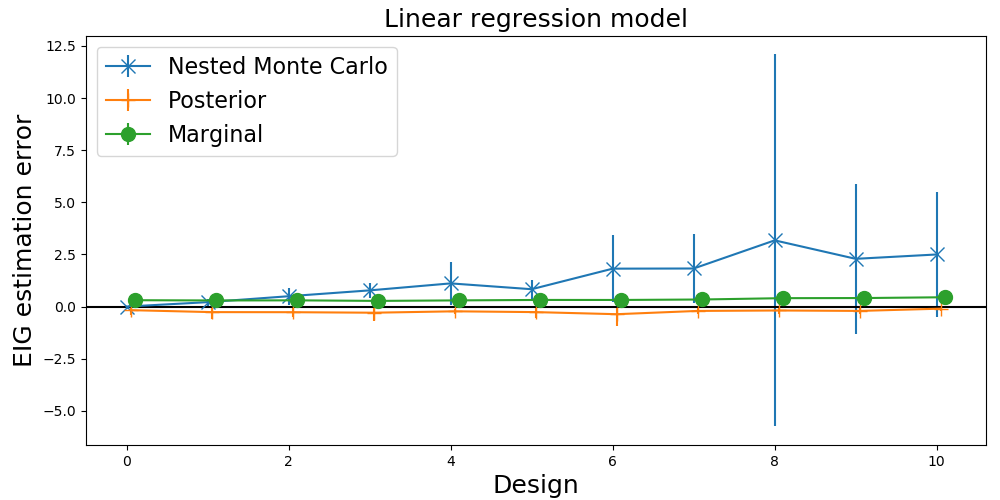
\includegraphics[scale=.5]{figures/lm.png}
	\end{center}
	\caption{LinReg: EIG estimates for a linear regression model over 11 designs. We plot the mean and twice the standard deviation from 10 runs. Computational time was set to 10 seconds for comparison.}
	\label{fig:lm}
\end{figure}

\begin{figure}[h]
	\begin{center}
		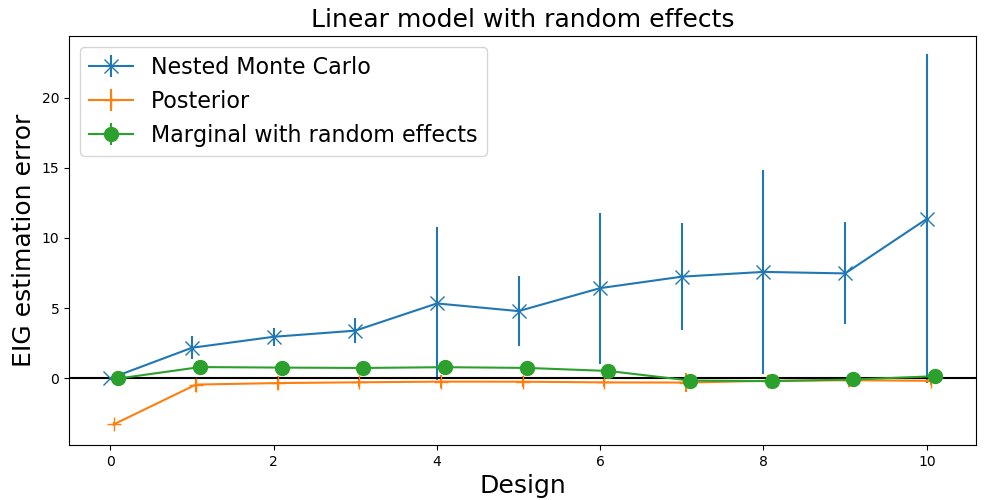
\includegraphics[scale=.5]{figures/lm_re.png}
	\end{center}
	\caption{LinReg + RE: EIG estimates for a linear regression model with random effects. Settings as in Figure~\ref{fig:lm}.}
	\label{fig:lm_re}
\end{figure}

\begin{figure}[h]\centering
	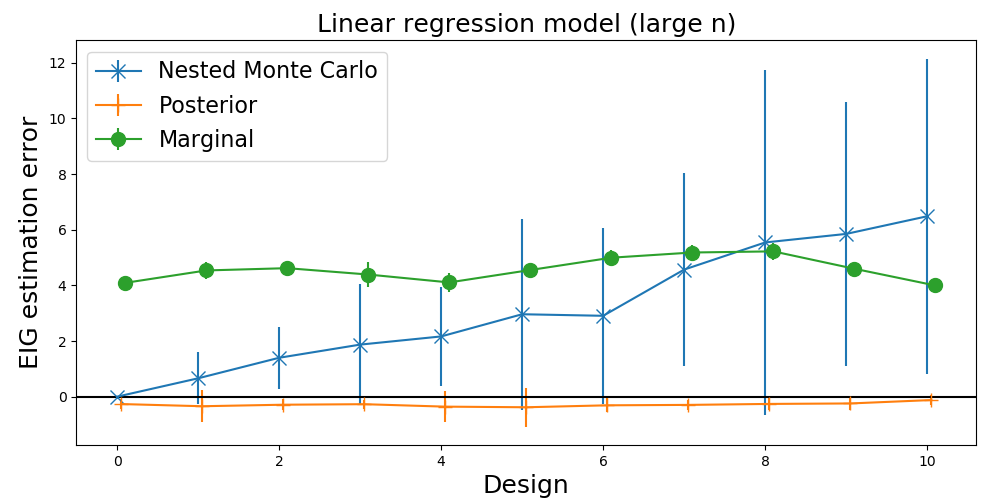
\includegraphics[scale=.5]{figures/lm_large_n.png}
	\caption{LinReg large ${\rm dim}(y)$: with settings as in Figure~\ref{fig:lm}.}
	\label{fig:largen}
\end{figure}

\begin{figure}[h]
	\begin{center}
		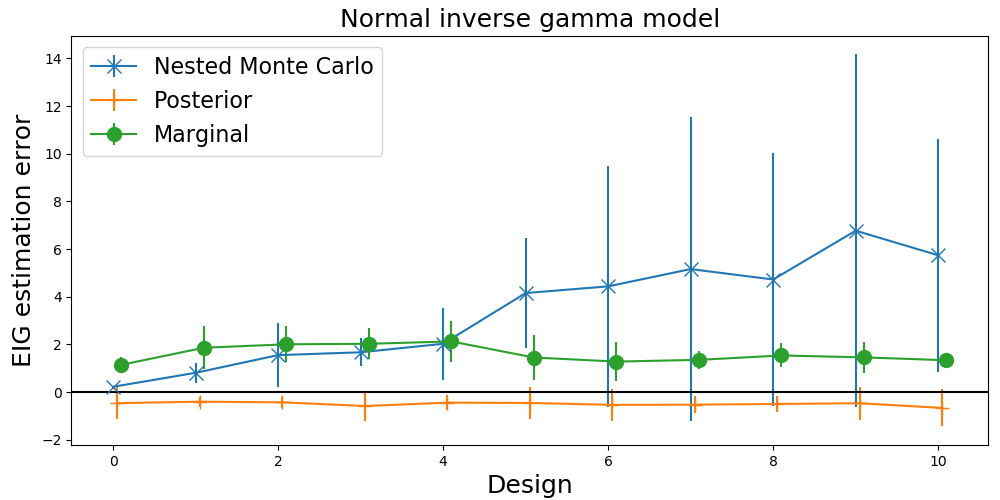
\includegraphics[scale=.5]{figures/nig.png}
	\end{center}
	\caption{N$\Gamma^{-1}$Reg: EIG estimates for a Normal inverse-Gamma model. Settings as in Figure~\ref{fig:lm}.}
	\label{fig:nig}
\end{figure}


\section{Extensions}
\subsection{Donsker-Varadhan}
The bounds in Section~\ref{sec:bounds} are partly inspired by the first bound described in Section~\ref{sec:mie}. We also considered using bounds based upon the Donsker-Varadhan representation, mentioned in the same section. The Donsker-Varadhan representation gives
\begin{equation}
	\label{eq:dveig}
	\eig(d) \le \expect_{p(y,\theta|d)} [T_d(y, \theta)] - \log\left(\expect_{p(\theta)p(y|d)}[e^{T_d(y,\theta)}] \right)
\end{equation}
Recall that the optimising $T_d$ is given by
\begin{equation}
	T_d^*(y, \theta) = \log\frac{p(y,\theta|d)}{p(y|d)p(\theta)} + C \text{ where }C\text{ is any constant.}
\end{equation}
Whilst direction comparison between Donsker-Varadhan our previously proposed methods is difficult if $T_d$ is a generic neural network, we can instead try either of
\begin{align}
	\label{eq:dvpost}
	T_{p, d} =& \log \frac{\qp(\theta | y,d)}{p(\theta)} \\
	T_{m, d} =& \log \frac{p(y|\theta,d)}{\qm(y|d)}
\end{align}
where $\qp$ and $\qm$ are the variational densities of Section~\ref{sec:bounds}. The form of $T_d^*$ guarantees that the Donsker-Varadhan bound will be tight under the same conditions that give tightness in the bounds of the previous section.

When compared, the Donsker-Varadhan bound fared poorly against the simpler bounds in experiments. A single evaluation of the bound required many more samples to be numerically stable.


\subsection{Analytic entropy}
Our proposed method is based on taking Monte Carlo sums of log densities to approximate integrals such as
\begin{equation}
	\label{eq:crossentropyest}
	\ape(d) \approx -\iint p(y, \theta | d) \log \qp (\theta | y, d; \phi)\, dy\, d\theta,
\end{equation}
which can be rewritten as
\begin{equation}
	\ape(d) \approx -\int p(y|d) \int p(\theta | y, d) \log \qp (\theta | y, d; \phi)\, d\theta\, dy
\end{equation}
we could instead have used the following
\begin{equation}
	\ape(d) \approx -\int p(y|d) \int \qp (\theta | y, d; \phi) \log \qp (\theta | y, d; \phi)\, d\theta\, dy = -\int p(y|d) \entropy{\qp (\theta | y, d; \phi)} dy.
\end{equation}
If the variational family $\mathcal{Q}$ for $\qp$ had been chosen so that $\entropy{\qp (\theta | y, d; \phi)}$ is easily calculable, the new approximation may have significantly lower Monte Carlo estimation error.

On the other hand, the new approximation does not bound $\ape(d)$ and so an entirely different mechanism to \textit{learn} $\qp$ must be employed. A correct learning approach is suggested by \cite{piera2009}, which showed that if $\kl{q_n}{p} \to 0$ then $\entropy{q_n} \to \entropy{p}$. In experiments, we trained $\qp$ using \eqref{eq:maxpost} just as in the original method. We used the analytic entropy in the final step.

In practice, most computation time was spent learning $\qp$ rather than making the final Monte Carlo estimate and so the gains from this alternative were negligible. 


\subsection{Experiments}
We compare the two suggested extensions against the posterior method of Section~\ref{sec:voed}. We used the same settings as the LinReg example. The biases and variances can be seen in Table~\ref{tab:abserrors2} and Figure~\ref{fig:lm2}. We see poorer performance from Donsker-Varadhan and little to tell between posterior, and posterior using analytic entropy.

\begin{table}[h!]
\begin{center}
    \begin{tabu}{|c|[1pt]c|c|}    \hline
  & \multicolumn{2}{c|}{\small LinReg2}  \\  
  \hline
  & \small bias & \small 2std   \\
  \tabucline[1pt]{-}
    \small Posterior & \small -0.24 & \small 0.32  \\
    \small Posterior, with analytic entropy & \small -0.33 & 0.53 \\
   \small Donsker-Varadhan & \small -0.46  & \small 1.01 \\ \hline
    \end{tabu}
\end{center}
     \caption{Bias and variance (we report $2\sigma$) of EIG estimation averaged over 10 runs and 11 designs. Each method was run for 10 seconds. For more details on the models and experimental setup see Appendix~\ref{sec:expdeets}.
 \vspace{-10pt}}
     \label{tab:abserrors2}
\end{table}

\begin{figure}[h]
	\begin{center}
		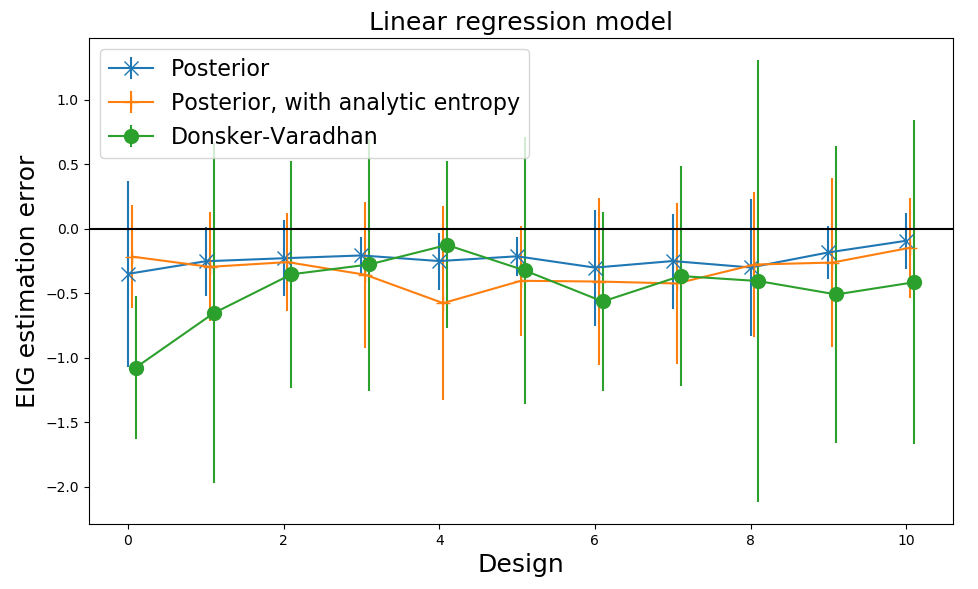
\includegraphics[scale=.5]{figures/ae_and_dv.png}
	\end{center}
	\caption{LinReg2: EIG estimates for a linear model, with extension methods. Settings as in Figure~\ref{fig:lm}.}
	\label{fig:lm2}
\end{figure}
